%%%%%%%%%%%%%%%%%%%%%%%%%%%%%%%%%%%%%%%%%
% Beamer Presentation
% LaTeX Template
% Version 1.0 (10/11/12)
%
% This template has been downloaded from:
% http://www.LaTeXTemplates.com
%
% License:
% CC BY-NC-SA 3.0 (http://creativecommons.org/licenses/by-nc-sa/3.0/)
%
%%%%%%%%%%%%%%%%%%%%%%%%%%%%%%%%%%%%%%%%%

%----------------------------------------------------------------------------------------
%	PACKAGES AND THEMES
%----------------------------------------------------------------------------------------

\documentclass{beamer}

\mode<presentation> {
%\usetheme{default}
%\usetheme{AnnArbor}
%\usetheme{Antibes}-
%\usetheme{Berkeley}
%\usetheme{Boadilla}
\usetheme{CambridgeUS}
%\usetheme{Copenhagen}
%\usetheme{Darmstadt}
%\usetheme{Dresden}
%\usetheme{Frankfurt}
%\usetheme{Goettingen}
%\usetheme{Hannover}
%\usetheme{Ilmenau}
%\usetheme{JuanLesPins}
%\usetheme{Luebeck}
%\usetheme{Madrid}
%\usetheme{Malmoe}
%\usetheme{Marburg}
%\usetheme{Montpellier}
%\usetheme{PaloAlto}
%\usetheme{Pittsburgh}
%\usetheme{Rochester}
%\usetheme{Singapore}
%\usetheme{Szeged}
%\usetheme{Warsaw}

\usecolortheme{seahorse}

\setbeamertemplate{navigation symbols}{}

}

\usepackage[spanish]{babel}
\usepackage[utf8]{inputenc}
\usepackage{graphicx}
\usepackage{booktabs}
\usepackage[spanish]{babel}
\usepackage{comment}
%----------------------------------------------------------------------------------------
%	TITLE PAGE
%----------------------------------------------------------------------------------------

\title[Gamificación]{Métodos y Técnicas de Gamificación Implementadas en Educación: Revisión Sistemática\\ Presentación de Avances} % The short title appears at the bottom of every slide, the full title is only on the title page

\author{Luis Angel Hernández Lázaro} % Your name
\institute[CIMAT] % Your institution as it will appear on the bottom of every slide, may be shorthand to save space
{
Centro de Investigación en Matemáticas A.C. Unidad Zacatecas \\ % Your institution for the title page
\medskip
\textit{luis.hernandez@cimat.com} % Your email address
}
\date{\today} % Date, can be changed to a custom date

\begin{document}

%----------------------------------------------------------------------------------------
%	PRESENTATION
%----------------------------------------------------------------------------------------
\begin{frame}
\titlepage
\end{frame}

\begin{frame}
\frametitle{Agenda}

\begin{columns}[c] % The "c" option specifies centered vertical alignment while the "t" option is used for top vertical alignment
	
	\column{.45\textwidth} % Left column and width
	\begin{figure}
		\begin{center}
			
\includegraphics[scale=0.25]{images/2icons/content.png}
		\end{center}
	\end{figure}
	
	\column{.5\textwidth} % Right column and width
	\tableofcontents 
	
\end{columns}
\end{frame}

%----------------------------------------------------------------------------------------
%	PRESENTATION SLIDES
%----------------------------------------------------------------------------------------

%------------------------------------------------
\section{Introducción} %
%------------------------------------------------

\begin{frame}
\Huge{\centerline{Introducción}}
\begin{figure}
	\begin{center}
		
\includegraphics[scale=0.2]{images/2icons/start.png}
	\end{center}
\end{figure}
\end{frame}

\begin{frame}
	\frametitle{Motivación}
	Elegí este tema debido al interés e el área para aplicar técnicas o métodos de gamificación en la educación, con el objetivo de motivar el aprendizaje de los estudiantes y mejorar su desempeño académico.
	\\~\\
	
	\begin{figure}
		\begin{center}
			
\includegraphics[scale=0.1]{images/2icons/student.png}
		\end{center}
	\end{figure}
\end{frame}

\begin{frame}
	\frametitle{BackGround}
	.\\~\\
\end{frame}

\section{Revisión Sistemática}
\begin{frame}
\Huge{\centerline{Revisión Sistemática}}
	\begin{figure}
		\begin{center}
			
\includegraphics[scale=0.4]{images/2icons/systematicReview.png}
		\end{center}
	\end{figure}
\end{frame}


\subsection{Proceso}
\begin{frame}
	\frametitle{El Proceso de la Revisión Sistemática}	
	\begin{figure}[H]
		\begin{center}
			
\includegraphics[scale=0.4]{images/1document/steps.png}
		\end{center}
	\end{figure}
	\begin{figure}[H]
		\begin{center}
			
\includegraphics[scale=1]{images/2icons/steps.png}
		\end{center}
	\end{figure}
	
\end{frame}


%------------------------------------------------
%------------------------------------------------
\subsection{Planeación de la Revisión}
\begin{frame}
\Huge{\centerline{Planeación de la Revisión}}
	\begin{figure}
		\begin{center}
			
\includegraphics[scale=.4]{images/2icons/plan.png}
		\end{center}
	\end{figure}
\end{frame}

\begin{frame}
    \frametitle{Protocolo}    .
	\begin{figure}
		\begin{center}
			
\includegraphics[scale=0.1]{images/2icons/need.png}
		\end{center}
	\end{figure}
\end{frame}

\begin{frame}
    \frametitle{Identificación de la Necesidad de la Revisión Sistemática}
    Hoy en día la Gamificación es un tema que esta siendo aplicado más allá de los juegos que tradicionalmente conocemos, la aplicación de técnicas para gamificación pueden ser variadas dependiendo del área donde se trabaje. Entonces, es importante conocer si las técnicas y métodos de Gamificación desarrollados para la educación pueden ser aplicados en entornos de la educación en línea (E-Learning).
\end{frame}

\begin{frame}
	\frametitle{Objetivos: General y Específicos (1/2)}
	Como parte de la definición de nuestro Objetivo General del estudio tenemos:
	\begin{description}
		\item[Definir] el estado del arte actual del uso de técnicas de Gamificación en la educación tradicional (Aula, Alumno, Profesor), para descubrir las diferentes técnicas de Gamificación implementadas en la educación.
	\end{description}
	\begin{figure}
		\begin{center}
			
\includegraphics[scale=0.1]{images/2icons/tarjet.png}
		\end{center}
	\end{figure}
\end{frame}

\begin{frame}
	\frametitle{Objetivos: General y Específicos(2/2)}
	Los objetivos Específicos del estudio son:
	\begin{description}
		\item[Definir] el estado del arte de la Gamificación en la educación.
		\item[Revisar] las estrategias o técnicas de Gamificación implementadas en el área de la educación.
		\item[Comparar] la aplicación de técnicas de gamificación en la educación.
	\end{description}
	\begin{figure}
		\begin{center}
			
\includegraphics[scale=0.1]{images/2icons/tarjet2.png}
		\end{center}
	\end{figure}
\end{frame}


\begin{frame}
    \frametitle{Especificación de las Preguntas de Investigación}
    \begin{table}
                \begin{center}
                    \label{table:researchQuestions}
                    \begin{tabular}{| p{5.5cm} | p{5.5cm} |}
                        \hline
                        \multicolumn{1}{|c|}{\textbf{Pregunta}}  & \multicolumn{1}{|c|}{\textbf{Objetivo}} \\
                        \hline
                        ¿Qué elementos de gamificación son usados en la educación? & Identificar los elementos de Gamificación existentes, en particular en la educación. \\
                        \hline
                        ¿Qué tipo de estudios de investigación aplican gamificación en la educación? & Descubrir los trabajos que han sido desarrollados para aplicar la gamificación en la educación. \\
                        \hline
                        ¿Qué técnicas de gamificación han sido más efectivas? & De las técnicas existentes cuales han tenido resultados positivos en la educación y porque. \\
                        \hline
                        ¿La gamificación promueve el aprendizaje? & Verificar si el conocimiento de los estudiantes mejora con la aplicación de gamificación.\\
                        \hline
                        ¿En qué nivel educativo ha sido investigada la gamificación? & Conocer que experiencias se han tenido en el uso de gamificación.\\
                        \hline
                    \end{tabular}
                \end{center}
            \end{table}
\end{frame}

\begin{comment}
\begin{frame}
    \frametitle{Evaluación del Protocolo de Revisión}
    Como parte de la evaluación del protocolo se realizaron revisiones con la Dra. Mirna profesora de la materia de Estudio Guiado I y el Dr. Arturo asesor para el realizar este trabajo.\\
    Observaciones para evaluar el trabajo:
    \begin{itemize}
    	\item Actualización de la palabra clave  (KeyWord) ``Serious Game" por ``Serious Games".
    \end{itemize}
    \begin{figure}
    	\begin{center}
    		
\includegraphics[scale=.1]{images/2icons/checklist.png}
    	\end{center}
    \end{figure}
    
\end{frame}
\end{comment}
%------------------------------------------------
%------------------------------------------------
\subsection{Ejecución de la Revisión} %
\begin{frame}
\Huge{\centerline{Ejecución de la Revisión}}
	\begin{figure}[H]
		\begin{center}
		    
\includegraphics[scale=.3]{images/2icons/execute.png}
	    \end{center}
	\end{figure}
\end{frame}

\begin{frame}
	\frametitle{Selección de las Fuentes de Investigación (1/3)\\Palabras Clave}
	\begin{columns}[c] % The "c" option specifies centered vertical alignment while the "t" option is used for top vertical alignment
		\column{.5\textwidth} % Left column and width
		Definición de Palabras Clave:
		\begin{itemize}
			\item Gamification
			\item Gamify
			\item Serious Games
			\item Education
			\item E-Learning
		\end{itemize}
		\column{.3\textwidth} % Right column and width
		\begin{figure}
			\begin{center}
				
\includegraphics[scale=0.2]{images/2icons/keyword.png}
			\end{center}
		\end{figure}	    	
	\end{columns}
\end{frame}


\begin{frame}
	\frametitle{Selección de las Fuentes de Investigación (2/3)\\ Cadenas de Búsqueda}
	\begin{table}
		\begin{center}
			\begin{tabular}{| l | p{10cm} |}
				\hline
				\multicolumn{1}{|c|}{\textbf{Núm}} & \multicolumn{1}{|c|}{\textbf{Cadena de Búsqueda}} \\
				\hline
				SS1 & ( ``Gamification''{ }AND (``Education''{ }OR ``E-Learning''{ }) )\\
				\hline
				SS2 & ( ``Serious Games''{ }AND ``Gamification''{ }AND (``Education''{ }OR ``E-Learning''{ }) )\\
				\hline            
				SS3 & ( ``Gamify''{ }AND (``Education''{ }OR ``E-Learning''{ }) )\\
				\hline
			\end{tabular}
		\end{center}
	\end{table}
	    \begin{columns}[c]
	    	\column{.2\textwidth}
	    	\begin{figure}
	    		\begin{center}
	    			
\includegraphics[scale=.5]{images/2icons/r.png}
	    		\end{center}
	    	\end{figure}
	    	\column{.2\textwidth}
	    	\begin{figure}
	    		\begin{center}
	    			
\includegraphics[scale=0.1]{images/2icons/q.png}
	    		\end{center}
	    	\end{figure}
	    	\column{.2\textwidth}
	    	\begin{figure}
	    		\begin{center}
	    			
\includegraphics[scale=0.1]{images/2icons/rq.png}
	    		\end{center}
	    	\end{figure}
	    \end{columns}
\end{frame}

\begin{frame}
    \frametitle{Selección de las Fuentes de Investigación (3/3)\\ Bibliotecas Digitales}
    \begin{table}
    	\begin{center}
    		\begin{tabular}{| p{5cm} | p{5cm} |}
    			\hline
    			\textbf {Fuentes Contempladas en un Inicio} &  \textbf{Fuentes Donde se Realizó la Búsqueda}\\
    			\hline
    			IEEE Xplore Digital Library & IEEE Xplore Digital Library\\
    			\hline
    			ACM Digital Library & ACM Digital Library\\
    			\hline
    			Web of Science & Web of Science\\
    			\hline
    			JSTOR & x\\
    			\hline
    			Scopus & Scopus\\
    			\hline
    			Springer Link & Springer Link\\
    			\hline
    			Elsevier Science Direct & Elsevier Science Direct\\
    			\hline
    			Google Scholar & x\\
    			\hline
    		\end{tabular}
    	\end{center}
    \end{table}
    \begin{columns}[c]
    	\column{.2\textwidth}
    	\begin{figure}
    		\begin{center}
    			
\includegraphics[scale=1.2]{images/2icons/library.png}
    		\end{center}
    	\end{figure}
    	\column{.2\textwidth}
    	\begin{figure}
    		\begin{center}
    			
\includegraphics[scale=0.2]{images/2icons/books.png}
    		\end{center}
    	\end{figure}
    \end{columns}
\end{frame}


\begin{frame}
    \frametitle{Procedimiento de Selección de Estudios\\ Criterios de Inclusión y Exclusión}
	
	\begin{table}
		\begin{center}
			\begin{tabular}{| p{5.5cm} | p{5.5cm} |}
				\hline
				\multicolumn{1}{|c|}{\textbf{Criterios de Inclusión}} & \multicolumn{1}{|c|}{\textbf{Criterios de Exclusión}} \\
				\hline
				Incluir artículos donde el título contengan dos palabras clave de nuestras cadenas de búsqueda principalmente ``Gamification''{ }& Excluir todos los artículos donde el título no contengan las palabras clave de la cadena de búsqueda.\\
				\hline
				Incluir artículos donde el resumen presente una relación con la aplicación de técnicas de  gamificación. & Excluir artículos donde el resumen no tenga relación con la aplicación de técnicas de gamificación.\\
				\hline
				Incluir artículos que estén escritos en Ingles y Español. & Excluir artículos que no estén en los idiomas del criterio de inclusión.\\ \hline
				Incluir artículos entre el rango de años: 2010 - 2015. & Excluir artículos publicados menores al año 2010.\\
				\hline
			\end{tabular}
		\end{center}
	\end{table}
\end{frame}

\begin{frame}
    \frametitle{Evaluación de la Calidad de Estudios\\ Criterios de inclusión y exclusión aplicados para la calidad del Estudio}
    .\begin{table}
    	\begin{center}
    		\begin{tabular}{| p{6cm} | p{4cm} |}
    			\hline
    			\multicolumn{1}{|c|}{\textbf{Criterios de Inclusión}} & \multicolumn{1}{|c|}{\textbf{Criterios de Exclusión}} \\
    			\hline
    			Incluir información sobre métodos de implementación para establecer estrategias de aprendizaje por medio de ``Gamification''.{ }& Excluir toda la información que no este relacionada con los criterios de inclusión definidos.\\
    			\hline
    			Incluir información que contenga experiencias del aprendizaje con ``Gamification''. &{.} \\
    			\hline
    			Incluir información donde se muestren estudios para el aprendizaje por medio de técnicas de e-learning.& {.}\\ \hline
    		\end{tabular}
    	\end{center}
    \end{table}
\end{frame}

\begin{frame}
    \frametitle{Extracción y Monitoreo de la Información}
    \footnotesize
        	    \begin{table}
        	    	\begin{center}
        	    		\begin{tabular}{| l | p{7cm} |}
        	    			\hline
        	    			\multicolumn{2}{|c|}{\textbf{REGISTRO DE ARTÍCULO}} \\ \hline
							NÚMERO & Identificador Propio \\ \hline
        	    			TÍTULO & Titulo del Artículo \\ \hline
        	    			CATEGORÍA & Gamification, Education, E-Learning, Serious Games \\ \hline
        	    			AÑO DE PUBLICACIÓN & Año de Publicación del Artículo \\ \hline
        	    			\begin{tabular}[c]{@{}l@{}}PALABRAS CLAVE \\ (KEYWORDS)\end{tabular} & Lista de Palabras Clave del Artículo \\ \hline
        	    			ABSTRACT & Resumen del Artículo \\ \hline
        	    			\begin{tabular}[c]{@{}l@{}}NOTAS ACERCA\\ DEL ABSTRACT \end{tabular} & Ideas principales del resumen del Artículo \\ \hline
        	    			\multicolumn{2}{|c|}{\textbf{EXTRACCIÓN DE LA INFORMACIÓN}} \\ \hline                        
        	    			\begin{tabular}[c]{@{}l@{}}RESUMEN DE\\ SECCIONES\end{tabular} & Estructura del documento con ideas principales de cada sección.\\ \hline
        	    			\begin{tabular}[c]{@{}l@{}}TÉCNICAS, MÉTODOS,\\ APLICACIONES;\\ CREADAS\end{tabular} & Descripción de las Técnicas, Métodos o Aplicaciones para el uso de Gamificación.\\ \hline
        	    			NOTAS  ADICIONALES & Material Extra e ideas para comprender el estudio.\\ \hline
        	    		\end{tabular}
        	    	\end{center}
        	    \end{table}	
\end{frame}


\begin{frame}
	\frametitle{Resumen Selección Estudios Primarios}
	\begin{figure}
		\begin{center}
			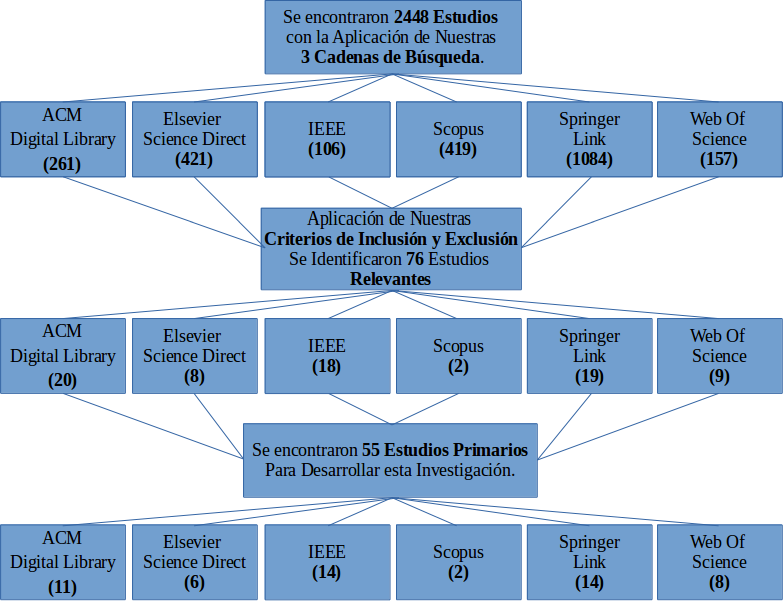
\includegraphics[scale=0.35]{images/1document/results.png}
		\end{center}
	\end{figure}
\end{frame}

\begin{frame}
    \frametitle{Sístensis de la Información}
    .
	\begin{figure}
		\begin{center}
			
\includegraphics[scale=0.45]{images/2icons/need.png}
			
		\end{center}
	\end{figure}
\end{frame}

%------------------------------------------------
\subsection{Reporte de Resultados} %
%------------------------------------------------

\begin{frame}
\Huge{\centerline{Reporte de Resultados}}
\end{frame}

\begin{frame}
    \frametitle{Métodos y Técnicas Aplicados}
    .
	\begin{figure}
		\begin{center}
			
\includegraphics[scale=0.45]{images/2icons/need.png}
			
		\end{center}
	\end{figure}
\end{frame}

\begin{frame}
    \frametitle{Evaluación del Reporte}
    .
	\begin{figure}
		\begin{center}
			
\includegraphics[scale=0.45]{images/2icons/need.png}
			
		\end{center}
	\end{figure}
\end{frame}
%------------------------------------------------
\section{Conclusiones} %
%------------------------------------------------
\begin{frame}
    \frametitle{Conclusiones}
    .
	\begin{figure}
		\begin{center}
			
\includegraphics[scale=0.45]{images/2icons/need.png}
			
		\end{center}
	\end{figure}
\end{frame}
%------------------------------------------------

\begin{frame}
\frametitle{References}
\footnotesize{
\begin{thebibliography}{99} % Beamer does not support BibTeX so references must be inserted manually as below
\bibitem[Smith, 2012]{p1} John Smith (2012)
\newblock Title of the publication
\newblock \emph{Journal Name} 12(3), 45 -- 678.
\end{thebibliography}
}
\end{frame}

%------------------------------------------------

\begin{frame}
\Huge{\centerline{The End}}
\end{frame}

%----------------------------------------------------------------------------------------

\end{document} 